% !Mode:: "TeX:UTF-8"
\chapter{移动社交网络中的关系识别分析}

关系识别是当前社交网络的重要研究课题之一。在一个社交网络中,人们会因为不同的关系而联系在一起,如家人、朋友、同事关系等等。明确社交网络中用户之间不同的关系类型,有利于其它领域的深入研究与发现。如在线或者移动广告营销中,如果知道用户家人、朋友的兴趣爱好以及其常购买的商品类型,那么就能更加准确的给该用户推荐相关的商品与广告,反之亦然,知道用户的喜好,也可以给其朋友、家人等推荐相应合适的商品。在协助公安侦破并抓捕犯罪嫌疑人时,如果能够掌握犯罪嫌疑人其家庭、朋友,则能更快协助相关部门侦破案件,有效的抓捕犯罪人员。由前面介绍可以得知,随着移动智能手机的大规模普及,移动通话数据的人群覆盖率已经接近100\%, 具有相当的普适性。除此之外,移动运营商所提供了家庭套餐、集团套餐等营销套餐,如果研究者能够和移动运营商进行合作,则研究者能够利用从移动运营商中获得的关系数据,作为其训练数据。

从第二章可以得知,从机器学习的角度来看,关系识别实质是一个分类问题。基于目前的研究现状,已经有相当多的学者对此进行了研究。但大多数此类研究都是将关系拆分为简单的“信任与不信任”,“强关系与弱关系”,“友好与敌对”关系,并没有将关系具体到一个明确的网络当中去(如具有家庭、同事、朋友的关系网)。还有部分研究对对关系分类赋予了特定的寓意,但这些研究主要有“指导-被指导(Advisor-Advisee)”\upcite{wang2010mining}、“讲授(Teaching)-指导(Advisor)-助教(Teaching Assistant)”关系\upcite{taskar2003link},比较适用于有向关系,而并非特别适合我们所研究的家庭、同事和朋友关系集。另外一些研究则是基于特别的数据集,如恐怖分子网络数据集分布\upcite{zhao2006entity}, 和我们所要进行研究的通话网络数据结构和性质相差太大,并且这些性质的研究,大多仅从社交层面上对关系进行阐释,而不能从模型的角度充分挖掘社交与空间地理位置之间的联系,而我们所要做的工作则需要从这两个角度同时进行考虑。


移动社交网络提供了非常丰富的信息,可以用来挖掘人们在真实日常生活中的社交关系。在本章,我们首先对基于通话数据中移动社交网络的关系识别问题进行论述和定义,然后将我们所研究的数据进行详细介绍。最后,我们针对从用户通话角度、地理位置同现两个角度进行出发,研究不同交互特征下同事、家庭、朋友关系之间的显著差异,并对特征进行相应的分析。我们用通话数据展示我们的发现。由于篇幅的限制,我们不展示在短信息中的发现,但两者的特征发现比较相近。

\section{关系识别问题定义}
很显然,社交网络是一个图模型,因此不同的问题的基本构成都可以用图$G = (V, E, W)$来进行表示,其中网络图中的每个点$ v_i \in V$表示该网络中的用户,图中点与点的边$Edge(v_i, v_j) \in E$ 表示用户$i$与用户$j$之间存在某种联系(这种联系可以自己定义,如在我们的问题中即两人存在社交关系),而$W$则表示了这种点与点之间的关系强度(如在我们的问题中,则可以定量描述为两用户之间的通话频率与强度等)。

具体到我们的问题当中,我们让$G = (V, E, X, Y)$ 代表无向移动社交网络,这里的$V$ 是$|V| = N$数量的用户集合,而$E \subset V \times V$是表示用户之间社交联系边的集合,每一条边$e_i \in E$ 都有一个相应的社交关系$y_i \in Y$与之对应,这里的$Y \in $\{家庭关系, 同事关系,朋友关系\}。需要注意的是,这里的朋友关系定义为联系较为频繁的用户。$\textbf{X}$是特征矩阵,$\bm{x_i}$代表了$|\bm{x_i}|$维特征向量,为每条边$e_i$的特征。因此在解决最终问题,推断移动社交网络前,我们需要选取合适的特征,即$\bm{x_i}$的值。



\section{数据介绍}
在本论文中所使用的数据集是从2010年10月1日到2010年10月25日采集的中国河南省某县级市的移动手机通话短信数据,包含了30万用户超过六千万(67,630,000)条的通话记录,三千万(31,560,000)条的短信记录,四百万(4,420,000)条的手机开关机纪录,一千二百万条的基站切换纪录。该县级市总共有354座基站,而且每一座基站都有相应的经度和纬度。其中通话、短信的格式如表3.1,开机关机、基站切换的纪录格式如表3.2.




除此之外,我们还有由移动运营商提供的家庭集团和同事工作集团的数据。为了更加精确、更加合理的预测用户之间的关系类别,我们移除了那些家庭集团和工作集团大小为1的孤立点,因为这些点不会对我们所分析的问题构成任何贡献(我们研究的问题本身就是边的关系)。除去这些无用的用户之后,我们可以发现大多数的集团由两个或者三个构成,这类型的集团占了所有家庭和同事集团总数的83\%。并且我们从数据分布上可以发现,同时集团的大小大多小于10人。


\begin{table}
    \centering
    \caption{短信/通话记录格式}
    \label{call-record}
    \begin{tabular}{c|c|c|c|c}
        \hline
        主叫号码 & 被叫号码 & 通话时长 & 主叫基站 & 被叫基站 \\ \hline
        1597128XXXX & 1565295XXXX & 2010-10-20 18:12:34 & 60234 & 60183 \\ \hline
    \end{tabular}
\end{table}


\begin{table}
    \centering
    \caption{事件纪录格式}
    \label{event-record}
    \begin{tabular}{c|c|c|c|c}
    \hline
    事件发生时间 & 用户手机号码 & 时间类型 & 起始基站 & 终止基站 \\ \hline
    2011-10-20 10:10:13   & 135XXXXXXX & 1 & 60284 & 74856  \\ \hline
    \end{tabular}
\end{table}


\begin{figure}[ht]
    \centering
    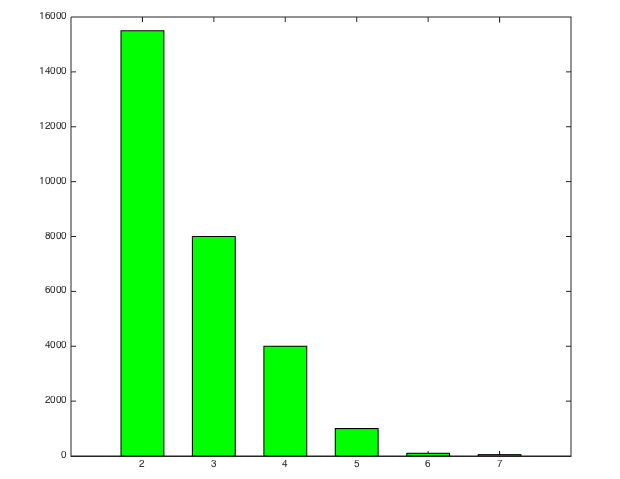
\includegraphics[scale=1,width=0.7\textwidth]{figure/FamilyClique.png}
    \caption{家庭集团大小分布}
    \label{fig-familyclique}
\end{figure}

\begin{figure}[ht]
    \centering
    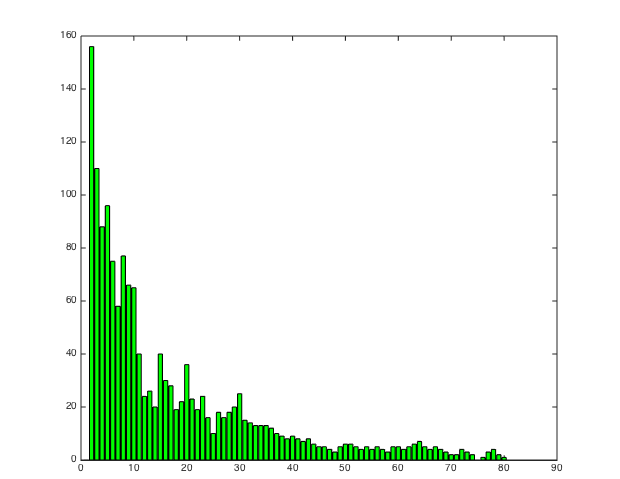
\includegraphics[scale=1,width=0.7\textwidth]{figure/ColleagueClique.png}
    \caption{同事集团大小分布}
    \label{fig-colleagueclique}
\end{figure}



\section{社交关系识别中的特征分析}

本节主要从移动社交网络中的用户交互、时空交互、社交与时机地理空间交互等角度来分析影响社交关系识别的关键特征,充分利用移动社交网络的社交、空间结合等特性。本小节先从通话社交的角度进行分析,主要分析基本的通话特征对关系识别的影响,以及引入通话熵的概念,然后分析不同关系用户之间时间和通话强度的稳定性与差异性。然后从时空交互的角度来分析,分析了用户时空同现性。随后,分析用户出现地理位置的寓意分析,了解用户同现所在实际位置的具体含义。最后,从经典的社交结构论扩充到地理空间的范围内,提出新的结构洞理论。

\subsection{基本社交通话特征行为分析}

从以前的研究中,我们可以知道,通过用户的通话记录,用户之间的关系(朋友、非朋友)能够很好的被识别出来\upcite{min2013mining}。但在那篇文章所用到的数据集都非常的小,并不能代表用户交互之间公共的特点,并不能直接认为围绕通话记录所得到的通话特征行为在我们的数据集上也有同样的效果。因此,我们在我们文章的数据集中重新考虑了用户之间的通话记录对关系识别的影响。

在图3.3中,我们分析了不同的社交关系在一天之内,不同小时段的通话概率分布情况。这里我们定义忙时为每天的10AM到12AM,6PM到9PM期间。可以看到,无论哪儿种关系,在通话整体分布上呈现双峰分布,而曲线的最高点即为每天的忙时期间。在图中我们不难发现到,那些具有家庭关系的用户会比具有同事关系的用户拥有更高的交流通话频率。除此之外,我们也可以观察到,家人之间往往会选择在忙时进行通话。而具有同事关系的用户,往往选择的是在工作时间段(每天的9点到12点,以及下午14点到18点)内进行通话,而到了下班时间,我们会选择与具有家庭关系的用户进行通话,很有可能要通知家人是否要回去吃晚餐,大概几点会到家等话题。另外,朋友关系并不具有很明显的时间段分布,这反映了朋友关系往往是有事了才会选择通话,而并不具有每日特定时段的规律性,反映了朋友通话的随机性。从中我们可以知道,不同社交关系在不同时段之间的通话关系在一定程度上,反映了我们日常的行为,如从上述分析中我们可以知道人们往往会在下班之后选择和家人进行通话。这也充分反映了通话行为在识别不同社交关系的有效性。



\begin{figure}[ht]
    \centering
    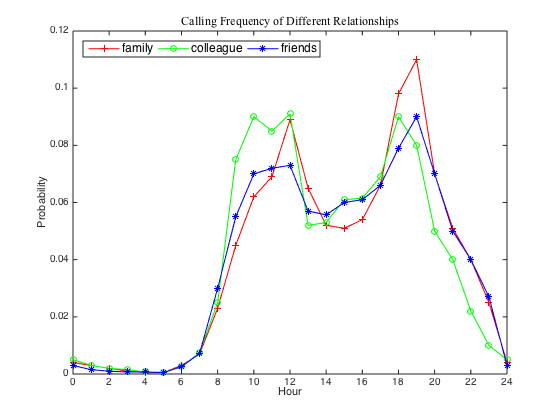
\includegraphics[scale=1,width=0.8\textwidth]{figure/callFrequencyDistribution.png}
    \caption{社交关系与不同小时段通话频率之间的联系}
    \label{fig-callFrequency}
\end{figure}

从日常生活经验中,我们可以知道,人们在周末和工作日的通话行为往往是不一样的,为此,有必要分析不同社交关系在工作日和周末的通话行为。如图3.4,图(a)为在工作日的不同社交关系通话频率分布差异,图(b)为在周末不同社交关系的通话频率分布差异。除了在上述图3.3的分析中所发现的特性,我们分析工作日和周末通话频率的共性和差异可以知道,无论是周末还是工作日,具有家庭关系的用户的通话频率都远远的超过具有同事或朋友关系的用户,这也充分体现了人们往往与自己的家人联系数量最多、最为紧密。同时,在周末,无论是具有家庭关系还是同事关系的用户,相对于工作日,两类关系的通话频率均有下降。这并不难发现,在周末家人大多数时间都是呆在一块,并不需要通过电话来进行联系。而同事之间在休息日若无工作,则很少通过电话来进行沟通。而朋友关系,正如在图3.3中所发现的,在周末和工作日的分布较为平稳,没有很大的区分,这也反映了朋友关系之间的稳定性。


\begin{figure}[!ht]
    \centering
    \subfigure[工作日通话频率分布]{
        \label{fig-call-weekday}
        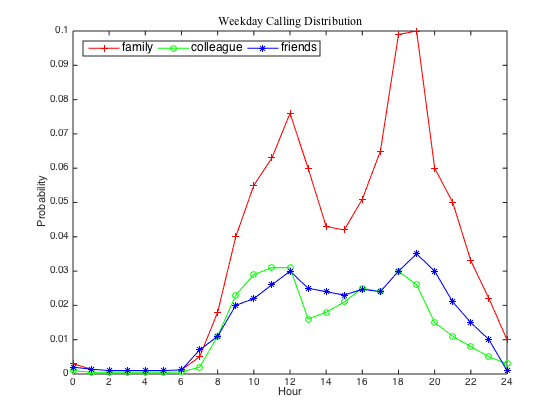
\includegraphics[width=.8\textwidth]{figure/callFrequencyWeekDayDistribution.png}
    }
    \hspace{7em} % 水平间隔
    \subfigure[周末通话频率分布]{
        \label{fig-call-weekends}
        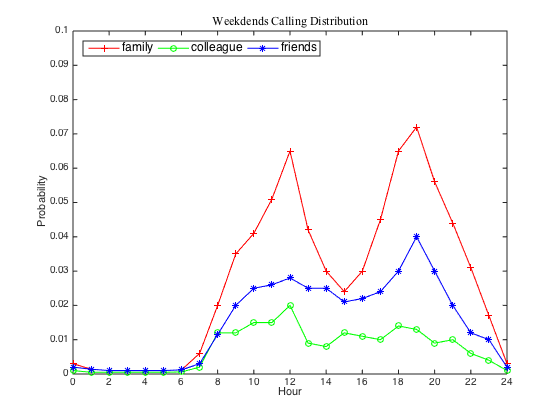
\includegraphics[width=.8\textwidth]{figure/callFrequencyWeekendsDistribution.png}
    }
    \caption{社交关系与不同小时段通话频率之间在工作日与周末的区别与联系}
    \label{fig-sub}
\end{figure}

\subsection{通话熵分布分析}

我们知道,我们会在不同的时间段内与不同的人通话联系。通常人们会在他们工作的时间与他们的同事通过手机联系。虽然说家人们主要集中在忙时通话,如下班之后。但是大多数的人们如果需要和他们的家人联系则不会等到某个特定的时间段内再联系,而是会直接打电话联系。为了定量描述这一特性,我们提出了通话熵的概念,可以用来描述用户之间通话的稳定性。熵的概念来源于信息领域,常常用来描述变量的随机性。由熵的概念而联想到的,我们定义了,通话熵的概念,用来描述通话在时间分布上的随机性。

\begin{definition}
    \label{call-entrpy-concept}
    \textbf{通话熵}计算公式,
    \begin{equation}
        CallEntropy = - \sum_{i=1}^{T}p(x_i)\cdot\log p(x_i)
    \end{equation}
\end{definition}


其中,$p(x_i)$ 代表了用户在第$i$小时段内通话的概率,$T$的值通常被设置为24,代表了一天里面有24小时。其计算结果代表了用户通话在一天内时间上的不确定性。如果通话熵的值比较小,那么用户的通话时间分布相对来说比较集中,这也意味着用户的通话时间分布相对比较稳定一些。反之,如果用户的通话熵越大,那么用户通话的时间越分散,即反映了该用户群体的通话时间越不确定。


\begin{figure}[!ht]
    \centering
    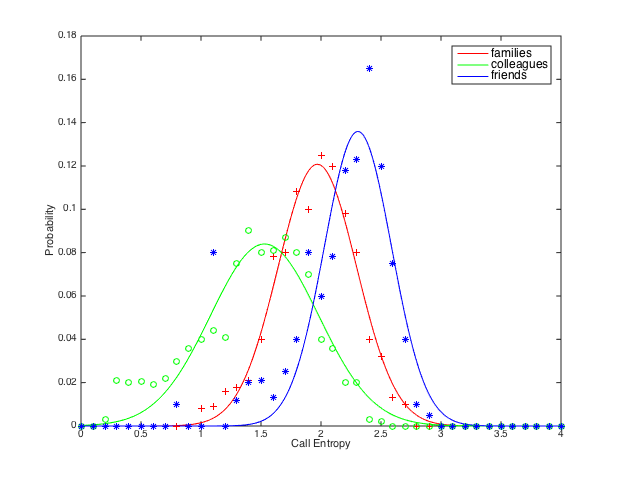
\includegraphics[scale=1,width=0.9\textwidth]{figure/CallEntropyDistribution.png}
    \caption{社交关系与通话熵之间的联系}
    \label{fig-call-entropy}
\end{figure}


在此概念的基础上,图3.5统计了不同社交关系用户的平均通话熵分布。我们可以发现基本上所有不同的社交关系的通话熵分布都遵循高斯分布。但是,具有朋友的社交关系的通话熵值是最大的,而具有家庭关系的用户的通话熵值小一些,而同事关系的通话熵值是最小的。这一现象揭示了同事之间往往会选择在特定的时间段(从前面的分析中我们可以知道主要在工作时间段内)进行通话,而家人和朋友则更多会随意一些。这也充分证明了朋友关系是作为一种非常重要的社交关系,因为人们在想起了事情或者想朋友了就会随时给他们打电话。这一区分度非常符合我们在实际生活中的通话习惯,以及处理不同社交关系的基本策略等等。

\subsection{空间位置同现性分析}

与传统的社交网络相比,移动社交网络不仅仅能够揭示用户之间基本通话行为所具有的特性,更能够从他们的地理位置分布等角度来挖掘新的特性。在我们的数据中,正如前面所介绍的,每一次用户的通话和短信,开关手机时,用户所在最近的基站都被记录了下来。由此,我们就能够得到用户每次呼叫的地理位置信息。基于这一其它社交网络并不具备的优势,我们进行分析不同社交关系与他们所具有的空间特征之间的联系时,具有得天独厚的条件。

在进行空间特征分析之前,我们需要分析我们的移动通话数据在多大程度上可以用来刻画用户在空间上的行为特征。为此,我们需要从数据集中所有带有地理位置信息的事件(短信、通话、基站切换、开关机等等)计算所有记录前后的时间差,以此确定用户出行行为规律。如图\ref{fig-position-stamp},我们统计了用户的位置间隔分布,可以看出,绝大多数的用户记录间隔都在一个小时之内,这也表明我们的数据集记录比较频繁,可以用来研究用户的出行行为。

\begin{figure}[ht]
    \centering
    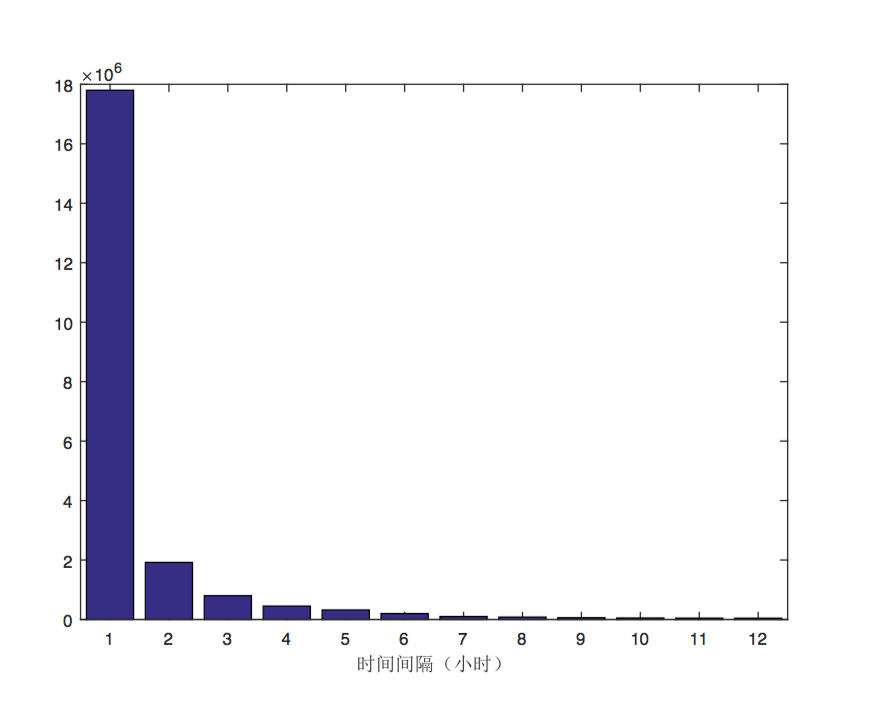
\includegraphics[scale=1, width=0.7\textwidth]{figure/timestamp.PNG}
    \caption{数据集中的用户位置间隔}
    \label{fig-position-stamp}
\end{figure}


接下来我们对用户的位置同现条件进行定义。这里的位置同现不同于字面上理解的两人在同一时刻出现在了同一地点,因这一类的数据在整个数据集上的分布较少,同时我们也无法确定同一地点的具体含义,因此我们需要重新定义同一时刻,即时间相邻的时间段,以及统一地点,即空间相邻的地理范围。在以前的研究中,以小时为时间粒度进行聚合,算作时间相邻,算是一种比较有效的手段\upcite{wang2011human}。另外考虑空间相邻的定义,为了得到用户的地理位置,我们往往是考虑用户所使用的基站的位置,因此只要两个不同的用户使用同一个基站,就可以认为他们在空间上具有位置同现的特性。但是,在真实世界中,因为有的地方基站分布较为密集,即是两个人处于确切的同一位置,他们也有可能暴露给两个不同的基站,因此很有必要合并一些距离非常近的基站。因基站合并算法在当前研究中较为成熟\upcite{aurenhammer1991voronoi},我们采用现成的算法,不再进行研究,直接使用大多数研究中所使用的基于$Voronio$ 图的基站临近合并算法\upcite{aurenhammer1991voronoi}。在进行这些工作之后,如果两个用户在一小时的时间间隔内处于同一基站下(合并之后的基站),那么我们可以认为,这两个用户时空位置同现。
























































